\documentclass{beamer}
\usepackage[spanish]{babel}
\usepackage[dvipsnames]{xcolor}
\usepackage{tikz}
\usepackage{hyperref}
%Declaracion del tema modificado
\usetheme[logo=rpi]{arturo}
%Declaracion de contenedor de imagenes
\graphicspath{{images/}}
%--------------------------------------
\title{Curso básico-intermedio de programación en Raspberry Pi}
\subtitle{Curso intersemestral}
\date{\today}
\author[OACM]{M.I. Omar Arturo Castillo Méndez} 

\begin{document}
	
	\begin{frame}[plain]
		\titlepage
	\end{frame}
	
	\begin{frame}{Contenido}
		\tableofcontents
	\end{frame}
	
	\section{Introducción}
	
	\begin{frame}{Introducción}
		\framesubtitle{Examen de diagnostico}
		\begin{itemize}
			\item ¿Qué es una tarjeta Raspberry Pi?
			\item Si conoces algún lenguaje de programación, ¿Cuál o cuáles?
			\item ¿Qué es el lenguaje de programación Python?
			\item ¿Qué bibliotecas de Python conoces?
			\item En la configuración de puertos de una RPi, ¿Qué diferencia hay entre el BCM y BOARD?
			\item Escriba un código para encender un LED en una tarjeta Raspberry Pi usando la configuración de puertos BOARD.
			\item ¿Cuáles son tus expectativas del curso?
		\end{itemize}
	\end{frame}
	\subsection{Generalidades y requisitos}
	\begin{frame}
		\frametitle{Introducción}
		\framesubtitle{¿Qué es una Raspberry Pi?}
		Es una tarjeta de desarrollo, diseñada como una computadora modular con una arquitectura ARM y usando un sistema operativo basado en Linux (Raspbian OS).
		\begin{figure}
			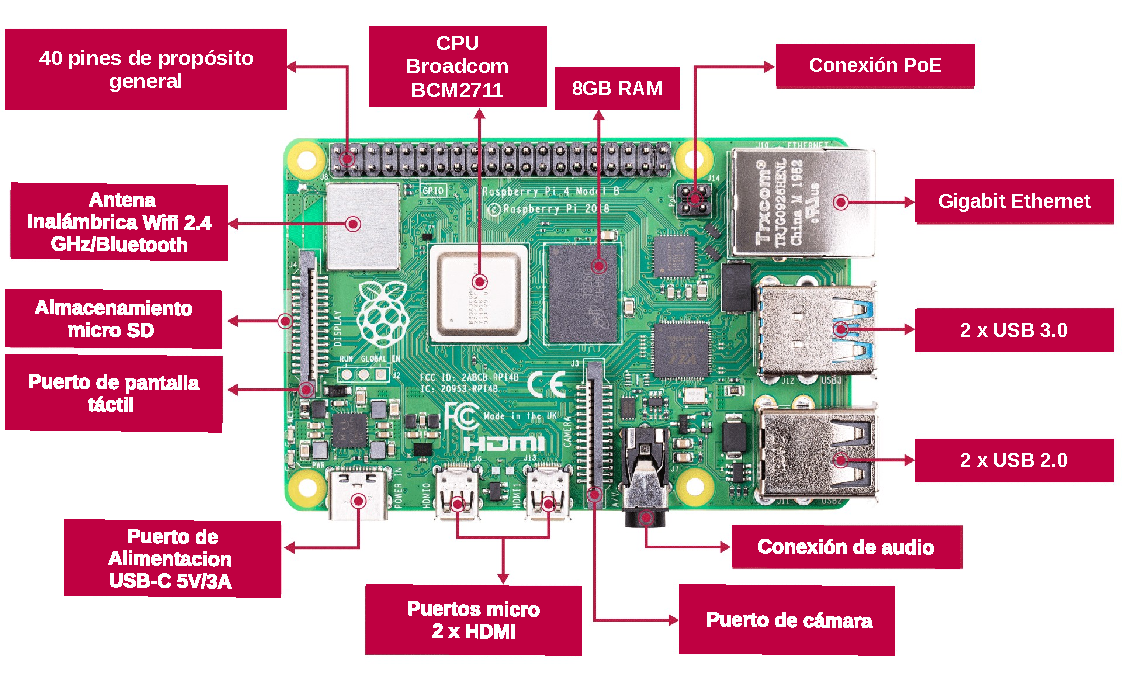
\includegraphics[scale=0.4]{rpiboard}
			\caption{Tarjeta Raspberry Pi 4}
		\end{figure}
		
	\end{frame}	

	\section{Configuración}
	\begin{frame}
		\frametitle{Configuración inicial}
		\framesubtitle{Requisitos}
		
		\begin{mybox}{Material necesario:}
			\begin{itemize}
				\item Tarjeta Raspberry. Pi(Cualquier versión)
				\item Fuente de alimentación de 5V a 3A.
				\item Tarjeta de almacenamiento micro SD de 64 Gb o superior clase 10 o superior.
				\item Mouse y teclado.
			\end{itemize}
		\end{mybox}
		
			
	\end{frame}

	\begin{frame}
		\frametitle{Configuración inicial}
		\framesubtitle{Instalación de Raspbian}
		
		\begin{mybox}{Instrucciones:} 
				\begin{itemize}
					\item Visitar la siguiente liga: \url{https://www.raspberrypi.com/software/}
					\item Descargar la versión correspondiente con su respectivo sistema operativo, y dar click en \textbf{descargar}
					\item Una vez instalado se mostrará la siguiente interfaz de Raspberry Pi Imager.
				\end{itemize}
		\end{mybox}
		
		
	\end{frame}
	
	\begin{frame}
		\frametitle{Configuración inicial}
		\framesubtitle{Instalación de Raspbian}	
		
		\begin{figure}
			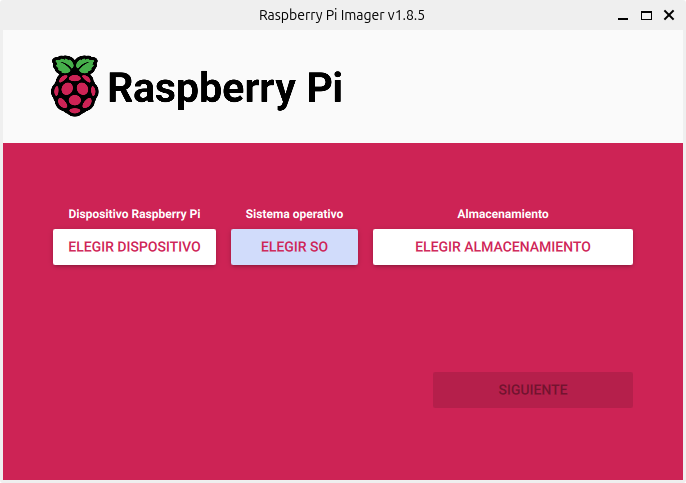
\includegraphics[scale=0.35]{imager.png}
			\caption{Interfaz: Raspberry Pi Imager}
		\end{figure}
		
	\end{frame}
	\subsection{Instalación de Raspbian}
	\begin{frame}
		\frametitle{Configuración inicial}
		\framesubtitle{Selección de Tarjeta}
		
		\begin{figure}
			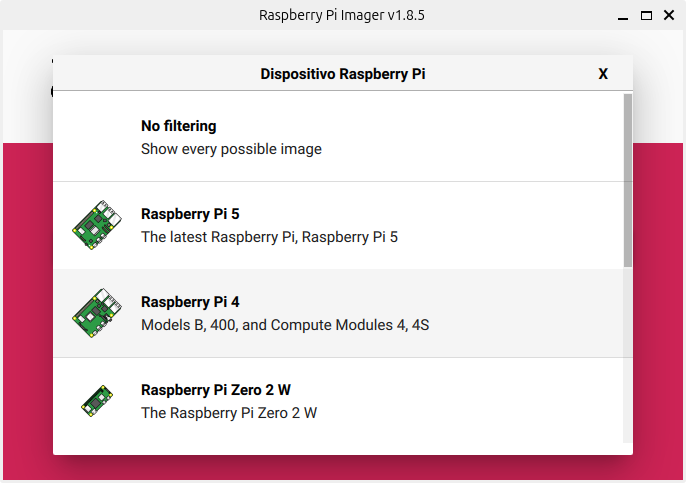
\includegraphics[scale=0.35]{imager2.png}
			\caption{Selección de tarjeta Raspberry Pi}
		\end{figure}
		
	\end{frame}
	
	\begin{frame}
		\frametitle{Configuración inicial}
		\framesubtitle{Selección de sistema operativo}
		
		\begin{figure}
			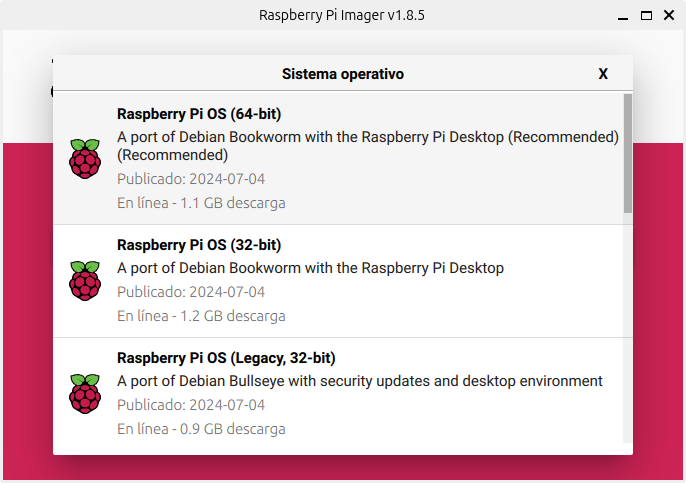
\includegraphics[scale=0.35]{imager3.png}
			\caption{Selección de sistema operativo}
		\end{figure}
		
	\end{frame}
	
	\begin{frame}
		\frametitle{Configuración inicial}
		\framesubtitle{Selección de unidad de almacenamiento}
		
		\begin{figure}
			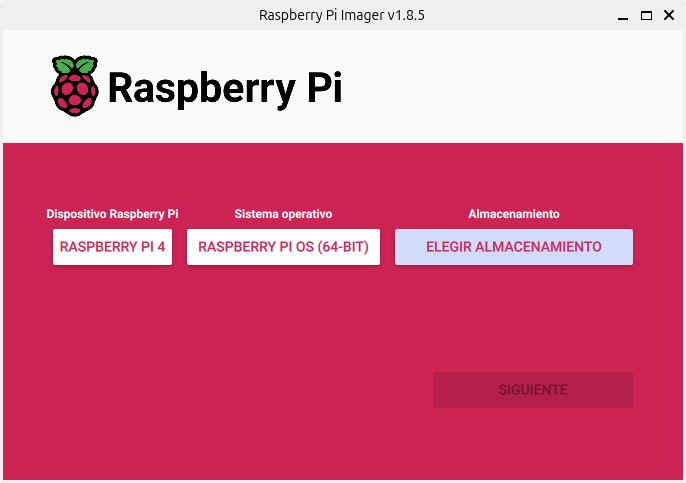
\includegraphics[scale=0.35]{imager4.png}
			\caption{Selección de unidad de almacenamiento}
		\end{figure}
		
	\end{frame}
	\subsection{Comandos básicos}
	\begin{frame}
		\frametitle{Configuración inicial}
		\framesubtitle{Comandos básicos de la terminal}
		\begin{mybox}{Instrucciones:}
			\begin{itemize}
				\item sudo :  Comando para acceder a derechos de superusuario.
				\item cd  : Cambiar de directorio a una ruta especificada.
				\item cd .. : Subir un nivel en la ruta.
				\item ls  : Listar archivos de un fichero/carpeta.
				\item pwd : Mostrar la ruta del carpeta.
				\item mkdir : Crear una carpeta.
				\item nano : Editor de texto desde la terminal.
				\item cp   : Copiar fichero o archivo hacia una ruta especificada.
				
				
			\end{itemize}
		\end{mybox}
		
	\end{frame}
	
	\begin{frame}
		\frametitle{Configuración inicial}
		\framesubtitle{Comandos básicos de la terminal}
		\begin{mybox}{Instrucciones:}
			\begin{itemize}
				\item ifconfig : Consultar la información de las interfaces de red.
				\item sudo raspi-config : Entrar a la configuración de la Raspberry Pi
				\item pinout : Muestra la distribución de pines de la tarjeta.
			\end{itemize}
		\end{mybox}
		
		
	\end{frame}
	\subsection{Ajustes de tarjeta RPi}
	\begin{frame}
		\frametitle{Configuración inicial}
		\framesubtitle{Cambiar la configuración de la RPi}
		
		Una vez terminada la instalación, se abre una terminal y se ejecuta el siguiente comando date: 
		\begin{figure}
			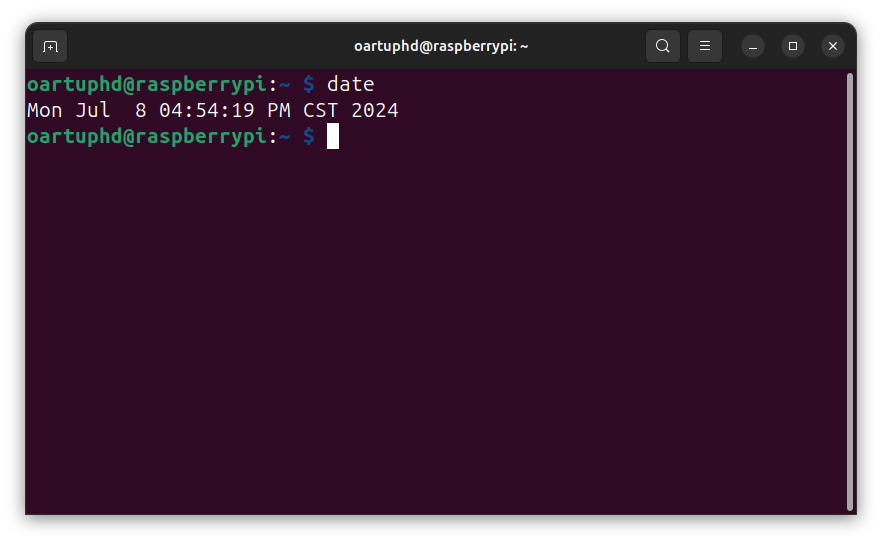
\includegraphics[scale=0.25]{daterpi.png}
			\caption{Consulta la fecha del sistema}
		\end{figure}
		Para colocar la fecha actual usar en la terminal de la RPi: \textbf{sudo date -s ‘YYYY-MM-DD HH:MM:SS'.}
		
	\end{frame}
	
	\begin{frame}
		\frametitle{Configuración inicial}
		\framesubtitle{Configuración de interfaces}
		Se ejecutará el siguiente comando: sudo raspi-config \newline
		Elegir la opción de \textbf{Interface Options}
		\begin{figure}
			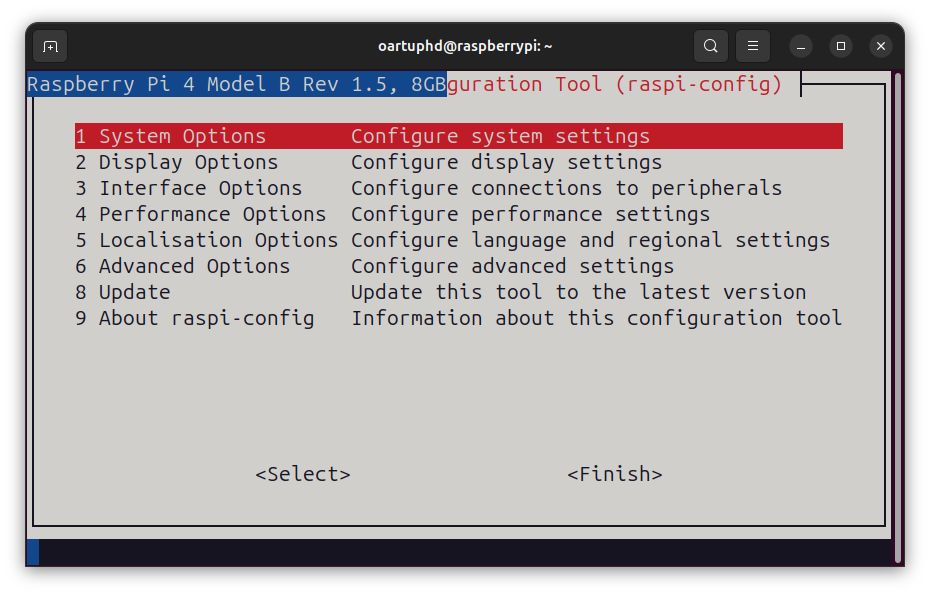
\includegraphics[scale=0.25]{configrpi.png}
			\caption{Opciones de configuración de la RPi}
		\end{figure}
	
		
	\end{frame}
	
		\begin{frame}
		\frametitle{Configuración inicial}
		\framesubtitle{Configuración de interfaces}
		Selecciona una por una las interfaces de SSH, SPI, I2C, Serial Port, 1-Wire.
		\begin{figure}
			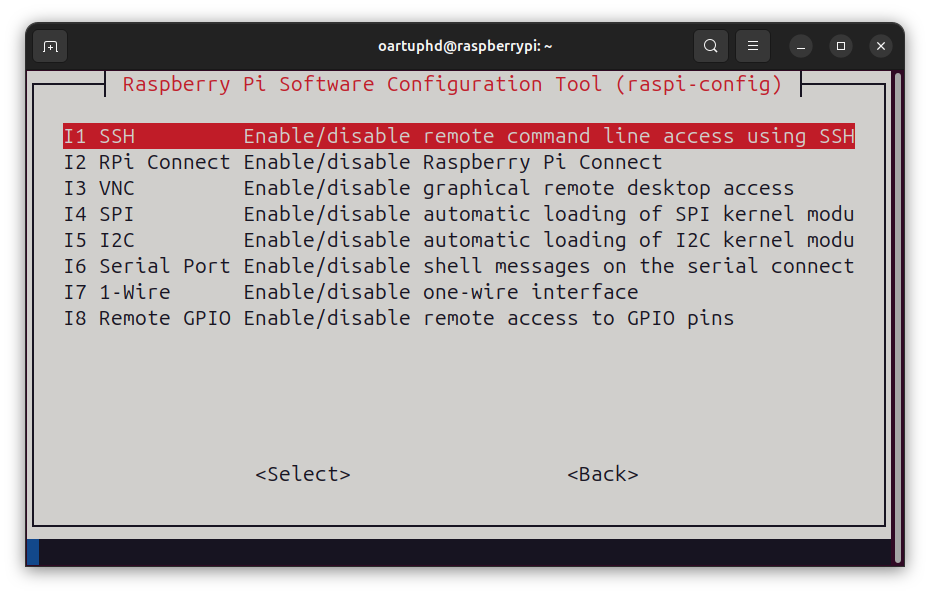
\includegraphics[scale=0.25]{configrpi2.png}
			\caption{Selección de interfaces de la tarjeta de RPi. }
		\end{figure}
		
	\end{frame}
	\subsection{Definición de IP estática}
	\begin{frame}
		\frametitle{Configuración inicial}
		\framesubtitle{Definir una IP estática}
		Para poder trabajar de manera remota sin la necesidad de usar un monitor externo mediante una terminal SSH(Secure Shell). Ejecutamos el siguiente comando en la terminal "\textbf{sudo nmtui} "
		
		\begin{figure}
			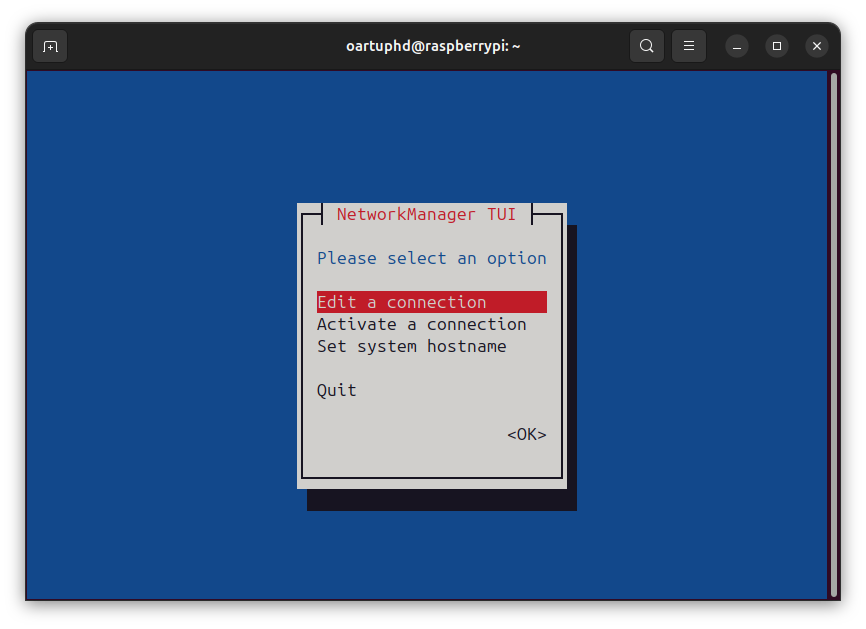
\includegraphics[scale=0.25]{rpissh.png}
			\caption{Administrador configuración de red.}
		\end{figure}
	\end{frame}
	\begin{frame}
	\frametitle{Configuración inicial}
	\framesubtitle{Definir una IP estática}
	Seleccionar el tipo de interfaz a convenir, si esta conectada vía Ethernet o Wi-Fi:
		\begin{figure}
			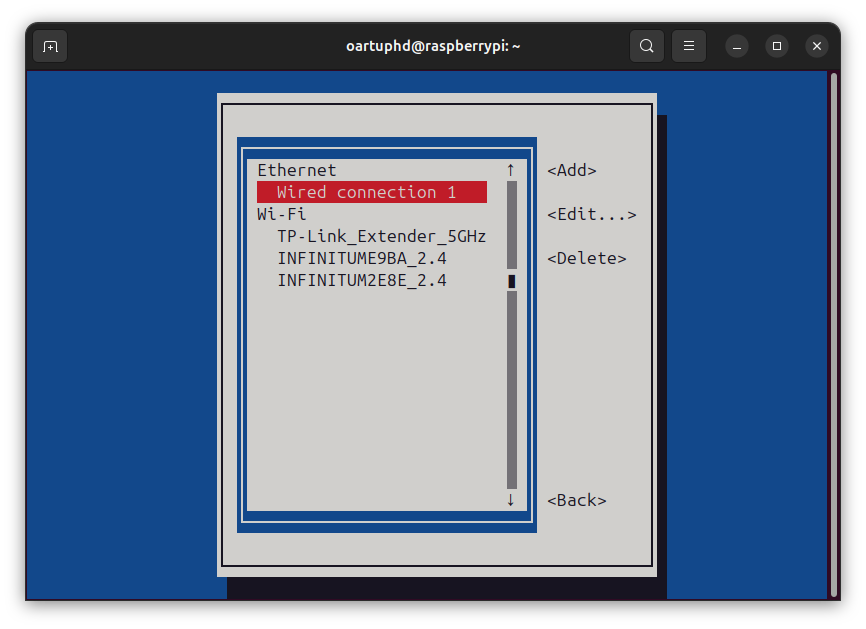
\includegraphics[scale=0.25]{rpissh2.png}
			\caption{Seleccionar la interfaz a modificar}
		\end{figure}
	\end{frame}
	
	\begin{frame}
		\frametitle{Configuración inicial}
		\framesubtitle{Definir una IP estática}
		En el apartado de IPv4 es donde se va a configurar la IP estática.
		\begin{figure}
			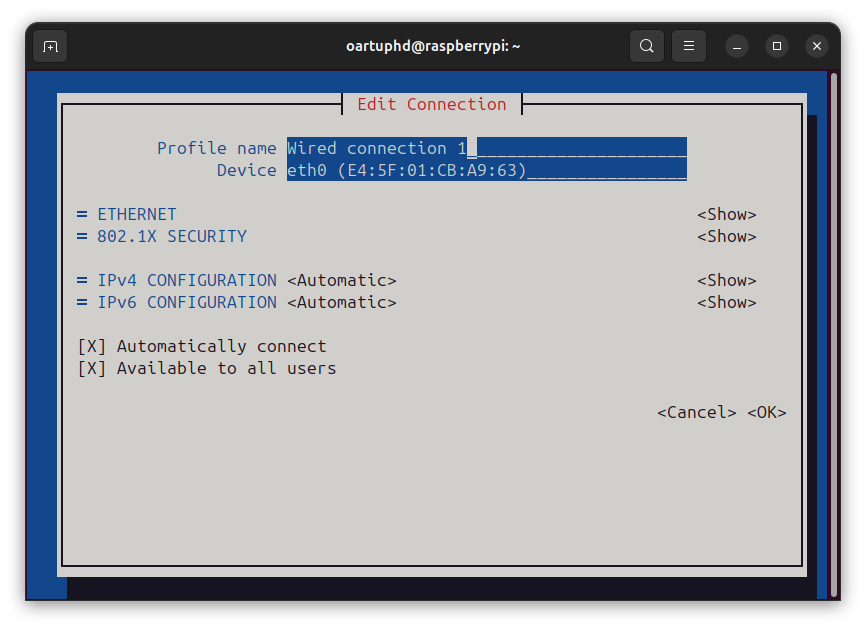
\includegraphics[scale=0.25]{rpissh3.png}
			\caption{Se seleccionó una conexión via Ethernet}
		\end{figure}
	\end{frame}
	\begin{frame}
		\frametitle{Configuración inicial}
		\framesubtitle{Definir una IP estática}
		Para consultar la IP a la cual esta conectada la RPi, vamos a salir del menú anterior y ejecutar en la terminal el siguiente comando: "\textbf{ifconfig}"
		
		\begin{figure}
			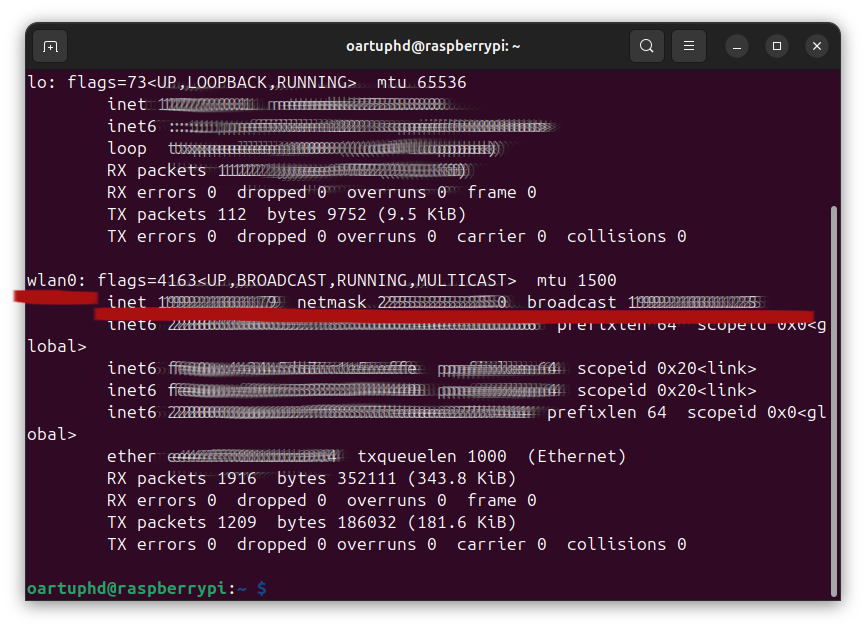
\includegraphics[scale=0.25]{rpissh5.png}
			\caption{Información de la red mediante el comando ifconfig}
		\end{figure}
		
	\end{frame}
	\begin{frame}
		\frametitle{Configuración inicial}
		\framesubtitle{Definir una IP estática}
		Una vez anotada la información anterior acceder el Network manager de la RPi, y capturar en: \textbf{Address}, \textbf{Gateway} y \textbf{DNS Server}
		\begin{figure}
			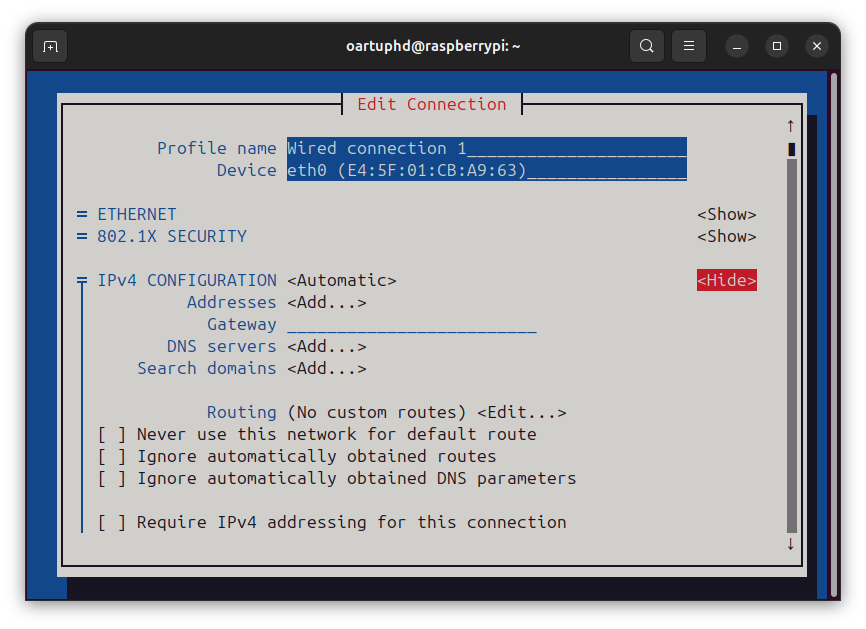
\includegraphics[scale=0.25]{rpissh4.png}
			\caption{Network manager de la RPi}
		\end{figure}
	\end{frame}
	\subsection{Conexión remota con SSH}
	\begin{frame}
		\frametitle{Configuración inicial}
		\framesubtitle{Conexion SSH con Windows}
		Para crear la conexión SSH con Windows se utilizará el siguiente programa PuTTY:
		\begin{mybox}{Instrucciones:}
			\begin{itemize}
				\item Visitar la siguiente liga: \url{https://putty.org/}
				\item Descargar la versión correspondiente con su respectivo sistema operativo.
				\item Seguir los pasos de instalación.
			\end{itemize}
		\end{mybox}
	\end{frame}
	\begin{frame}
		\frametitle{Configuración inicial}
		\framesubtitle{Conexión SSH con Windows}
		Terminada la instalación ubicar el programa PuTTY y ejecutarlo a continuación mostrará lo siguiente:
		\begin{figure}
			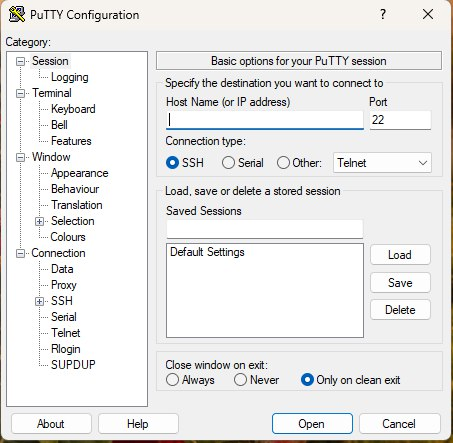
\includegraphics[scale=0.4]{putty.jpeg}
			\caption{Configuración de PuTTY}
		\end{figure}
		En el campo de \textbf{Host Name}, introducir la IP que previamente se fijo en la RPi.
	\end{frame}
	
	\begin{frame}
		\frametitle{Configuración inicial}
		\framesubtitle{Conexión SSH con Windows}
		Cuando se abra la terminal capturar el \textbf{usuario} que definieron al inicio de la instalación en Raspbian y su respectiva contraseña:
		\begin{figure}
			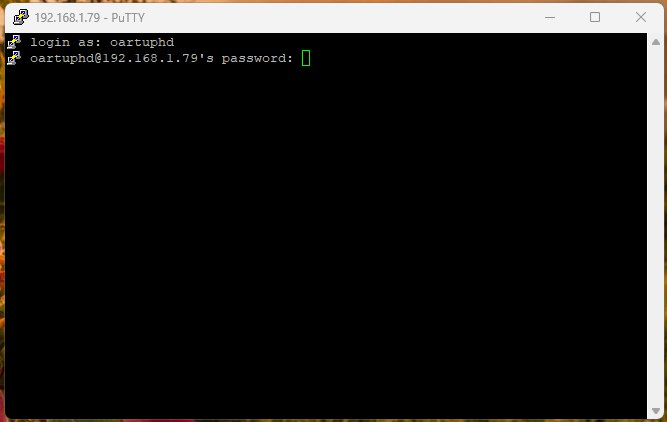
\includegraphics[scale=0.49]{putty2.jpeg}
			\caption{Captura de usuario y contraseña para acceso a la RPi}
		\end{figure}
		
	\end{frame}
	
	\begin{frame}
		\frametitle{Configuración inicial}
		\framesubtitle{Conexión SSH con Windows}
		Posteriormente aparecerá una advertencia de conexión aceptarla y finalmente aparecerá la terminal de la RPi:
		\begin{figure}
			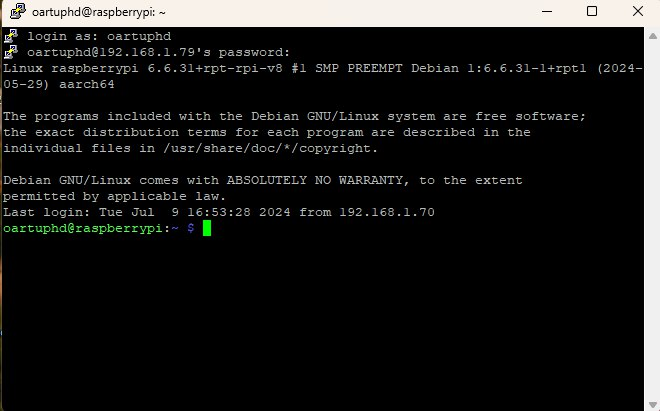
\includegraphics[scale=0.5]{putty3.jpeg}
			\caption{Terminal de la RPi}
		\end{figure}
		
	\end{frame}
	\subsection{Actualización de paquetes}
	\begin{frame}
		\frametitle{Configuración inicial}
		\framesubtitle{Actualización de paquetes}
		A continuación vamos actualizar todo el software instalado a la ultima versión usando el administrador de paquetes \textbf{apt} (Advanced Packaging Tool)
		\begin{mybox}{Comandos de actualización:}
			\begin{itemize}
				\item sudo apt update
				\item sudo apt upgrade
			\end{itemize}
		\end{mybox}
	\end{frame}
	\section{Programación en RPi}
	\begin{frame}
		\frametitle{Programación en RPi}
		\framesubtitle{Creación de un archivo}
		Para la creación de un archivo desde la terminal se tomaran los siguientes pasos:
		\begin{mybox}{Pasos a seguir:}
			\begin{itemize}
				\item Definir la ubicación donde estará la carpeta de trabajo (\textit{cd $\sim$/}).
				\item Crear la carpeta con el nombre a conveniencia (\textit{mkdir nombre-de-la-carpeta}).
				\item Usar el gestor de texto de la terminal para crear un archivo con extensión de Python(\textit{nano ejemplo.py}).
			\end{itemize}	
		\end{mybox}
	\end{frame}
	\begin{frame}
		\frametitle{Programación en RPi}
		\framesubtitle{Creación de un archivo}
		Con las instrucciones anteriores la terminal mostrará la siguiente ventana:
		\begin{figure}
			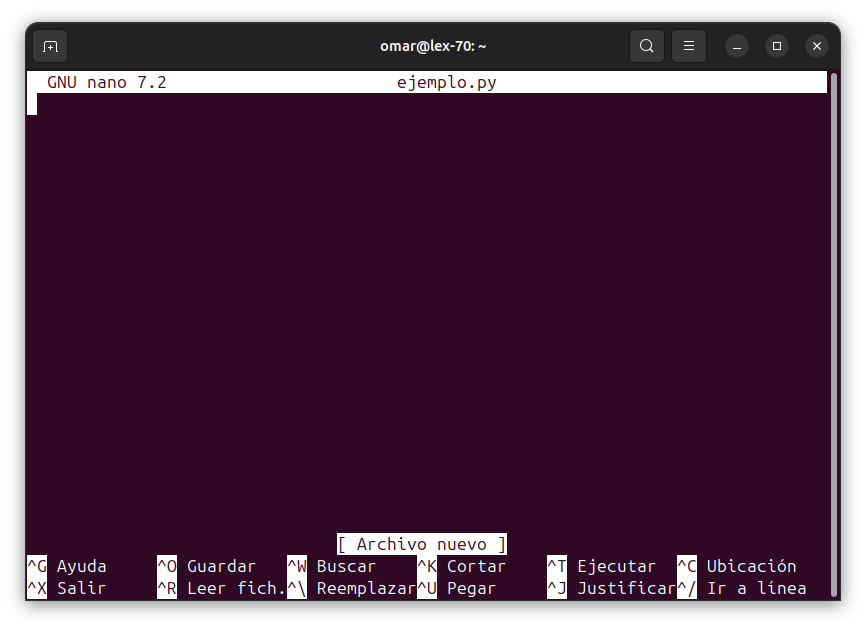
\includegraphics[scale=0.25]{nanorpi.png}
			\caption{Editor de texto nano. }
		\end{figure}
	\end{frame}
	\begin{frame}
		\frametitle{Programación en RPi}
		\framesubtitle{Actividad 1:}
		\begin{mybox}{Creación de un archivo de texto}
			\begin{itemize}
				\item Crear una carpeta en la dirección del \textit{home} con sus iniciales \textbf{abcd}, dentro de esa misma agregar otra carpeta con el nombre : \textbf{dia1}
				\item Dentro de la carpeta \textbf{dia1}, crear un archivo con la extension \textit{.txt}
				\item Con el editor de texto \textit{nano}, escribir una breve descripción de los comandos que se han utilizado hasta el momento.
			\end{itemize}
			
		\end{mybox}
	\end{frame}
	\subsection{GPIO}
	\begin{frame}
		\frametitle{Programación en RPi}
		\framesubtitle{¿Qué es el GPIO?}
		El GPIO o \textit{Entrada/Salidas de propósito general} es un pin genérico en un chip. En este caso la RPi cuenta con dos configuraciones de GPIO:
		\begin{mybox}{GPIO}
			\begin{itemize}
				\item GPIO.BOARD: Este indica a los pines según su numeración.
				\item GPIO.BCM: se refiere a los pines por su numero de \textit{Broadcom SOC channel}.
			\end{itemize}
		\end{mybox}
		Para mostrar los pines en la RPi se puede usar el comando \textit{pinout} en la terminal.
	\end{frame}
	\begin{frame}
		\frametitle{Programación en RPi}
		\framesubtitle{GPIO.BOARD}
		\begin{figure}
			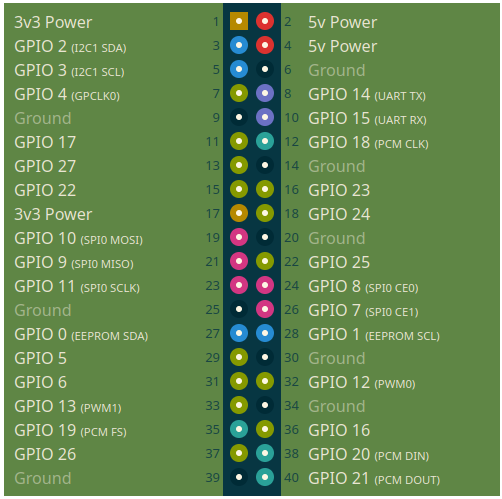
\includegraphics[scale=0.4]{rpiboard.png}
			\caption{Enumeración de pines según BOARD}
		\end{figure}
	\end{frame}
	\begin{frame}
		\frametitle{Programación en RPi}
		\framesubtitle{GPIO.BCM}
		\begin{figure}
			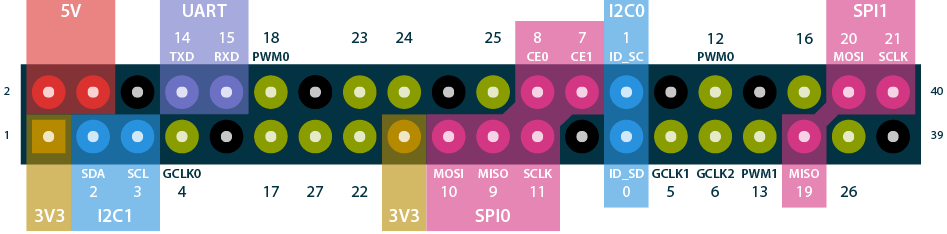
\includegraphics[scale=0.34]{rpibcm2.png}
			\caption{Enumeración de pines según BCM}
		\end{figure}
	\end{frame}
	\begin{frame}
		\frametitle{Programación en RPi}
		\framesubtitle{Uso del GPIO}
		Para el uso del GPIO usando Python vamos a programar lo siguiente:
		\begin{mybox}{Encender un LED}
			\begin{itemize}
				\item Se va encender y apagar un led con un retardo de 1 segundo.
				\item Uso de la biblioteca \textbf{time} y \textbf{GPIO.BOARD}
			\end{itemize}
		\end{mybox}
	\end{frame}
	\begin{frame}
		\frametitle{Programación en RPi}
		\framesubtitle{Uso del GPIO}
		\begin{figure}
			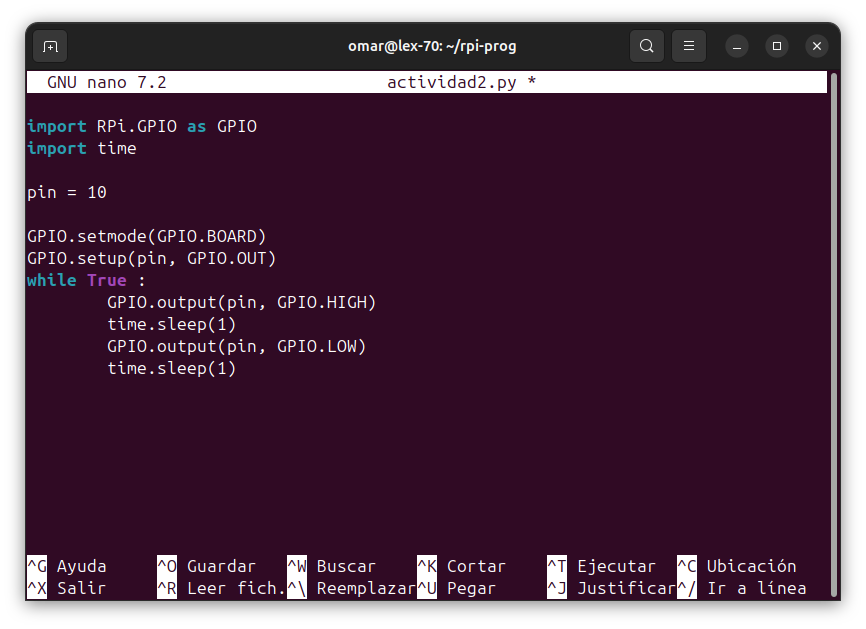
\includegraphics[scale=0.3]{led.png}
			\caption{Programa para encender un LED}
		\end{figure}
	\end{frame}
	\begin{frame}
		\frametitle{Programación en RPi}
		\framesubtitle{Actividad 2:}
		\begin{mybox}{Activación del GPIO}
			\begin{itemize}
				\item Crear un programa para controlar 3 LED.
				\item Con un retardo de 2 segundos entre cada LED.
				\item Usar la configuración del GPIO.BOARD.
				\item El archivo debe estar guardado en la carpeta que se creo anteriormente.
			\end{itemize}
		\end{mybox}
	\end{frame}
\subsection{Ambiente virtual venv}	
	\begin{frame}
		\frametitle{Programación en RPi}
		\framesubtitle{Instalación de venv}
		El modulo venv, admite la creación de entornos virtuales, sobre una instalación de Python existente y queda aislada para administrar de mejor manera la gestión de los paquetes que se instalan y evitar dañar la configuración actual. 
		\begin{mybox}{Instalación de venv}
			\begin{itemize}
				\item sudo apt install python3-venv
			\end{itemize}	
		\end{mybox}	
	\end{frame}
	
	\begin{frame}
		\frametitle{Programación en RPi}
		\framesubtitle{Configuración de venv}
		\begin{mybox}{Instalación de venv}
			\begin{itemize}
				\item Crear una carpeta donde ubicar el ambiente virtual
				\item Ejecutar para crear el ambiente virtual python -m venv nombredecarpeta
				\item Para activarlo source nombredecarpeta /bin/activate
				\item Para instalar un paquete nombredecarpeta/bin/pip install nombredebiblioteca
			\end{itemize}
		\end{mybox}	
	\end{frame}
	
		\begin{frame}
		\frametitle{Programación en RPi}
		\framesubtitle{Actividad 3:}
		\begin{mybox}{Instalacion de venv}
			\begin{itemize}
				\item Crear una carpeta dentro de \textbf{Documentos} con sus iniciales \textbf{abcd}
				\item Una vez creada su carpeta, dentro crear una nueva con el nombre de \textbf{virtual}
				\item Activar el ambiente venv en la terminal.
				\item Una vez activado, crear un archivo de texto \textbf{.txt} con los comandos utilizados al mismo nivel de su carpeta \textbf{abcd}
			\end{itemize}
		\end{mybox}
	\end{frame}
	
	\begin{frame}
		\frametitle{Programación en RPi}
		\framesubtitle{Sensor de temperatura: MLX90614}
		
		\begin{mybox}{Instalación de MLX90614}
			\begin{itemize}
				\item Visitar la dirección \url{https://pypi.org/project/PyMLX90614/}
				\item Instalar mediante pip con el ambiente virtual.
			\end{itemize}
		\end{mybox}
		
	\end{frame}
	
	
	
	\begin{frame}
		\frametitle{Programación en RPi}
		\framesubtitle{PWM}
		La modulación por ancho de pulso o PWM, se usa para controlar el ancho de una señal digital con el propósito de controlar a su vez la potencia que se entrega. Modificando el ancho del pulso activo.
		\begin{mybox}{Comandos para RPi}
			\begin{itemize}
				\item Se usará la biblioteca gpiozero basado en Python.
				\item Esta biblioteca genera una señal PWM por software.
				\item Los pines 0 y 1 estan restringidos para uso de PWM mediante la biblioteca.
			\end{itemize}
		\end{mybox}
	\end{frame}
	\begin{frame}
		\frametitle{Programación en RPi}
		\framesubtitle{PWM}
	\end{frame}
%----------------------------------------------------
\end{document}